\documentclass[12pt, oneside]{amsart}
\usepackage{amsmath}
\usepackage{lipsum}
\linespread{1.25}
\setlength{\topmargin}{0.in}
\setlength{\oddsidemargin}{0.33in}
\setlength{\textheight}{9.0in}
\setlength{\textwidth}{6.0in}
%-------Packages---------
\usepackage{amssymb,amsfonts}
\usepackage[all,arc]{xy}
\usepackage{enumerate}
\usepackage{mathrsfs}
\usepackage{graphicx}
\usepackage{epstopdf}
\usepackage{listings}
\usepackage{appendix}
\usepackage{listings}
\usepackage{placeins}
%\usepackage[square,numbers]{natbib}
\usepackage[style=apa,sortcites=true,sorting=nyt,backend=biber,natbib=true]{biblatex}
%bibliographystyle{unsrtnat}
\addbibresource{References/reference.bib}


%--------Theorem Environments--------
%theoremstyle{plain} --- default
\newtheorem{thm}{Theorem}[section]
\newtheorem{cor}[thm]{Corollary}
\newtheorem{prop}[thm]{Proposition}
\newtheorem{lem}[thm]{Lemma}
\newtheorem{conj}[thm]{Conjecture}
\newtheorem{quest}[thm]{Question}

\newtheorem{innercustomthm}{Theorem}
\newenvironment{customthm}[1]
  {\renewcommand\theinnercustomthm{#1}\innercustomthm}
  {\endinnercustomthm}

\theoremstyle{definition}
\newtheorem{defn}[thm]{Definition}
\newtheorem{defns}[thm]{Definitions}
\newtheorem{con}[thm]{Construction}
\newtheorem{exmp}[thm]{Example}
\newtheorem{exmps}[thm]{Examples}
\newtheorem{notn}[thm]{Notation}
\newtheorem{notns}[thm]{Notations}
\newtheorem{addm}[thm]{Addendum}
\newtheorem{exer}[thm]{Exercise}

\theoremstyle{remark}
\newtheorem{rem}[thm]{Remark}
\newtheorem{rems}[thm]{Remarks}
\newtheorem{warn}[thm]{Warning}
\newtheorem{sch}[thm]{Scholium}
\newcommand{\be}{\begin{equation}}
\newcommand{\ee}{\end{equation}}
\makeatletter
\let\c@equation\c@thm
\makeatother
\numberwithin{equation}{section}

%\bibliographystyle{plain}
%%%%%%%%%%%%%%%%%%%%%%%%%%%%%%%%%%%%%%%%%%%%%%%%%%%%%%%%%%%%%%%%%%%%%%%%%%%%%%%%%
% your title/author/date information go here
%--------Meta Data: Fill in your info------


\title{Cross-Validation Techniques for Auto-regressive Time Series}

\author{Xuan Li}

\date{September 8, 2024}

\begin{document}
\begin{abstract}
    This report is based on the paper titled "A Note on the Validity of Cross-Validation for Evaluating Autoregressive Time Series Prediction"\citep{Bergmeir2018}. This report is structured into three sections. The first section provides a comprehensive summary of the paper \citep{Bergmeir2018}, synthesizing its key findings and presenting the important points for a thorough understanding of the work. The second section presents two mini-proposals as possible extensional research projects beyond the original paper. The final section includes an extensional study we aim to explore. In specific, we aim to mimic similar experiments using auto-regressive time series data with lasso regression, comparing cross-validation methods with out-of-sample estimation. Additionally, the proof of Theorem 1 in the original paper in this extension scenario will be discussed from a general perspective.
\end{abstract}
\maketitle
\tableofcontents

%%%%%%%%%%%%%%%%%%%%%%%%%%%%%%%%%%%%%%%%%%%%%%%%%%%%%%%%%%%%%%%%%%%%%%%%%%%%%%%%%section 1

\section{Summary of the Original Paper}
The original paper explores the applicability of $K-fold$ cross-validation (CV) technique for evaluating auto-regressive time series models \citep{Bergmeir2018}. Cross-validation is widely used in machine learning type regression and classification tasks \citep{Hastie}. However, it is often considered problematic for time series data due to the serial correlation and non-stationarity \citep{Bergmeir2012}.  The authors demonstrated both theoretically and computationally that $K-fold$ CV can be valid and effective for auto-regressive models under certain conditions \citep{Bergmeir2018}.
\\

The paper builds on the existing literatures on model evaluation techniques for time series. Traditionally, out-of-sample ($OOS$) evaluation is preferred for time series due to concerns about using future data to predict the past, and issues with serial correlation in errors. In $OOS$, a block of data at the end of the set is left out as testing data, and the remaining data is used as training data. There are many studies that demonstrate this procedure in forecasting accuracy \citep{Tashman}. Previous studies have also proposed modifications to CV for dependent data \citep{Gyorfi, Burman1992, Burman1994}, such as $h-block$ CV, to account for dependence in time series data \citep{Burman1994}. In $h-block$ CV, $h$ data points preceding and following the observation are left out in the test set due to dependency. The authors of the original paper \citep{Bergmeir2018} referred to this type of CV as non-dependent cross-validation $nonDepCV$. However, this procedure often leads to inefficient use of data. The authors present their work as a shift from the usual thinking, arguing that under certain conditions, using standard $K-fold$ CV is not only valid but also helpful for auto-regressive models. In this case, the $K-fold$ CV can be used without modification, i.e., future data can be used as training data and past data can be used as testing data during this procedure. This is a key contribution, as it challenges the conventional thinking that CV is inappropriate for time series data. 
\\

The main idea is that the prediction error $\hat{PE}$ we get by performing cross validation methods on a data set $\{y_t\}_{t=1}^T$, will approximate the prediction error $PE$ when forecasting on the future data $\{y_t\}_{T+1}^n$ using past data set as the training data.  

\subsection{Theoretical Work}
The original paper provides a theoretical proof by showing that the prediction error in the in-set data performed by CV is a consistent estimator for the prediction error in the out-set data (the unseen future data). Without loss of generality, the paper focuses on the leave-one-out CV ($LOOCV$) because generalisation to the $K-fold$ CV is straightforward.
\\

Let $y_1, y_2, ..., y_n$ be a set of observation data from a stationary process. Let's consider a purely auto-regressive model of order $P$, i.e., AR(p), consider the following nonlinear regression model
\begin{equation}\label{eq1}
y_t = g(x_t, \theta) + \epsilon_t
\end{equation}

where $\epsilon_t$ is the regression error term, $x_t$ consists the lagged values of $y_t$ and $\theta$ is the parameter vector with all the coefficients values, and $g$ is the function of the lagged values of $y_t$ up to $p^{th}$ order.  $g$ is a continuous and differentiable function with respect to $\theta$ for all $x_t$ = $(y_{t-1}, y_{t-2}, ..., y_{t-p})'$. The estimation of $\hat{\theta}$ is the argument that minimises the objective function
\begin{equation}\label{eq2}
Q(\theta) = \sum_{t=p+1}^{n}
(y_t - g(x_t, \theta))^2
\end{equation}

Now suppose that $\{\Tilde{y_t}\}^m_{t=1}$ is another set of observations that has the same distribution as $\{{y_t}\}^n_{t=1}$, which can be the future data
\begin{equation}\label{eq3}
\Tilde{y_t} = g(\Tilde{x_t}, \theta) + \Tilde{\epsilon_t}
\end{equation}
The prediction error is defined as
\begin{equation}\label{eq4}
    PE = E(\Tilde{y} - g(\Tilde{x},\hat{\theta})^2
\end{equation}
where $\hat{\theta}$ here is the estimate minimizing the objective function $\tilde{Q}(\theta) = \sum_{t=p+1}^{m}
(\tilde{y}_t - g(\tilde{x}_t, \theta))^2$.
In the paper, the authors consider estimating $PE$ on dataset $\{\Tilde{y_t}\}^m_{t=1}$ by performing cross-validation on $\{y_t\}^n_{t=1}$. In the $LOOCV$ scene,  the training sample is $\{(x_j
, y_j); j = p+1,...,n, j \not = t\}$ and the test sample is $\{(x_t
, y_t)$\}. The estimator of $PE$ (denoted by $\hat{PE}$)  is defined as
\begin{equation}\label{eq5}
\hat{PE} = \frac{1}{n-p} \sum_{t=p+1}^n \left( y_t - g(x_t,\hat{\theta_{-t}}) \right)^2
\end{equation}
where $\hat{\theta_{-t}}$ is the leave-one-out estimate for $\theta$ on $\{(x_j, y_j); j = p+1,...,n, j \not = t\}$. In order to prove that $\hat{PE}$ approximates $PE$, the following assumptions are needed.

\newtheorem{assumption}{Assumption}
\begin{assumption}\label{assump1}
    The nonlinear AR(p) process that generated $\{{y_t}\}^n_{t=1}$ is stationary and ergotic.
\end{assumption}

\begin{assumption}\label{assump2}
    $\hat{\theta_{-t}}$ is a consistent estimator of $\theta$.
\end{assumption}


\begin{assumption}\label{assump3}
The errors are MDS: 
\begin{enumerate}
    \item $ \{ \epsilon_t,F_t \}$ form a sequence of martingale differences (MDS) where $F_t$ is the sigma field generated by $ \{ \epsilon_s, y_s;s \leq t \} $. Note that i.i.d errors are MDS.
    \item $Var(\epsilon_t | x_t) = \sigma^2$ and $E[|\epsilon_t|^{4+\delta} < K$ for some $K < \infty$ and $\delta > 0$.
    \item $\{\epsilon_t\}$ have absolutely continuous distribution with respect to Lebesgue measure. 
\end{enumerate}
\end{assumption}

Note that due to stationarity of $\{y_t\}^n_{t=1}$, conditions for the consistency of $\hat{\theta}$ and $\hat{\theta_{-t}}$ are equivalent. In short, we want to make sure that the time series model is stationary, the estimator is consistent, and the errors are uncorrelated.  \\

The theoretical validity is carried out by proving the following theorem. 

\begin{customthm}{1}\label{thm1}
Suppose that Assumptions \ref{assump1}-\ref{assump3} hold, then we have $\hat{PE} \xrightarrow[]{approx.} PE$. 
\end{customthm}
\begin{proof}
    
By expanding the prediction error into integral form, we have
$$PE = \int (\Tilde{y} - g(\Tilde{x},\hat{\theta}))^2 d\Tilde{F_m}$$
where $\Tilde{F_m}$ is the distribution of the process generating $\{\Tilde{y_t}\}^m_{t=1}$. Suppose the true model is $\Tilde{y} = g(\Tilde{x}, \theta) + \Tilde{\epsilon}$, where $g(\Tilde{x}, \theta)$ represents the true underlying relationship between $\Tilde{x}$ and $\Tilde{y}$, and $\Tilde{\epsilon}$ is the noise. By substituting for $\Tilde{y}$, we have 
$$PE = \int \left( g(\Tilde{x}, \theta) + \Tilde{\epsilon} - g(\Tilde{x},\hat{\theta}) \right)^2 d\Tilde{F_m}$$ By expanding the squared terms and simplification, we have 
$$PE = \int \left[ (g(\Tilde{x}, \theta) - g(\Tilde{x},\hat{\theta}))^2 + \Tilde{\epsilon}^ 2 \right] d\Tilde{F_m}$$

The authors performed a bias-variance decomposition by subtracting and adding the expected prediction $E[g(\Tilde{x}, \hat{\theta})]$, which represents the average prediction over multiple realizations of the training data. Therefore, we have 
$$ PE = \int \left[ \left(g(\Tilde{x}, \theta) - E[g(\Tilde{x}, \hat{\theta})] + E[g(\Tilde{x}, \hat{\theta})] - g(\Tilde{x},\hat{\theta})\right)^2 + \Tilde{\epsilon}^2 \right] d\Tilde{F_m}$$ By expanding the squared terms, we have

\begin{align*}
    PE &= \int \bigg[ \left(g(\tilde{x},\theta) - E[g(\tilde{x},\tilde{\theta})]\right)^2 + \left(E[g(\tilde{x},\tilde{\theta})] - g(\tilde{x}, \tilde{\theta})\right)^2 \\
    &+ 2 \left( g(\tilde{x}, \theta) - E[g(\tilde{x}, \hat{\theta})]\right) \left( g(\tilde{x},\hat{\theta}) - E[g(\tilde{x}, \hat{\theta})] \right) + \tilde{\epsilon}^2 \bigg] d\Tilde{F_m} 
\end{align*}

Notice that the cross-term vanishes when integrated since $E[ g(\tilde{x},\hat{\theta}) - E[g(\tilde{x},\hat{\theta}))] = 0$, and hence the equation can be simplified to
\begin{align*}
PE  &= \int \left[ \left(g(\Tilde{x}, \theta) - E[g(\Tilde{x}, \hat{\theta})] \right)^2 + \left(E[g(\Tilde{x}, \hat{\theta})] - g(\Tilde{x},\theta)\right)^2 + \Tilde{\epsilon}^2 \right] d\Tilde{F_m}\\ 
    &= \underbrace{\int  \left(g(\Tilde{x}, \theta) - E[g(\Tilde{x}, \hat{\theta})] \right)^2 d\Tilde{F_m}}_\text{Bias} + \underbrace{\int \left(E[g(\Tilde{x}, \hat{\theta})] - g(\Tilde{x},\hat{\theta})\right)^2 d\Tilde{F_m}}_\text{Variance} + \underbrace{\int \Tilde{\epsilon}^2  d\Tilde{F_m}}_\text{noise}\\  
\end{align*}
We expand $\hat{PE}$ in a similar vein. 
\begin{align*}
     \hat{PE} = \underbrace{\int  \left(g(x, \theta) - E[g(x, \hat{\theta_{-t}})] \right)^2 dF_n}_\text{Bias} + \underbrace{ \frac{1}{n-p}\sum_{t=p+1}^n \left( E[g(x_t, \hat{\theta_{-t}})] - g(x_t, \hat{\theta_{-t}}) \right)^2     }_\text{Variance} + \underbrace{\int \epsilon^2dF_n}_\text{noise}\\  
\end{align*}

where $F_n$ is the distribution of the process generating $\{y_t\}^n_{t=1}$. Notice that $\tilde{F_m}$ and $F_n$ are the empirical distributions of $2$ different samples from the same underlying process $F$, i.e $\{\Tilde{y_t}\}_{t=1}^m$ and $\{y_t\}_{t=1}^n$ are 2 datasets from the same underlying distribution process. By \textbf{Assumption \ref{assump1}} and \textbf{Assumption \ref{assump2}}, the underlying distribution process is stationary and ergotic, and  both $\hat{\theta}$ and $\hat{\theta_{-t}}$ are consistent estimators. The bias and noise terms in both $\hat{PE}$ and $PE$ are asymptotically identical. As $n, m \rightarrow \infty $, we want to show that

\begin{equation}\label{equation6}
   \frac{1}{n-p}\sum_{t=p+1}^n \left( E[g(x_t, \hat{\theta_{-t}})] - g(x_t, \hat{\theta_{-t}}) \right)^2 \xrightarrow{Approxi.} \int \left(E[g(\Tilde{x}, \hat{\theta})] - g(\Tilde{x},\hat{\theta})\right)^2 d\tilde{F_m} 
\end{equation}

The key takeaway here is that, ultimately, the variance of $PE$ across different training data realizations can be approximated by the variance of $\hat{PE}$ across different training data realizations when the number of data gets very big. When $n, m$ becomes big, let $N = max \{n, m\}$, and let $\epsilon^E_t(\hat{\theta_{-t}}) = E[g(x_t, \hat{\theta_{-t}})] - g(x_t,\hat{\theta_{-t}}), \tilde{\epsilon}^E_t(
\hat{\theta}
) = E[g(\Tilde{x_t}, \hat{\theta})] - g(\Tilde{x_t},\hat{\theta})$, we can write the left term in equation \ref{equation6} as
$$  \frac{1}{N-p} \sum_{t=p+1}^N  \left( \epsilon^E_t(\theta_{-t}) \right)^2$$and similarly we can write the right term as $$  \frac{1}{(N-p)^2} \sum_{t=p+1}^N \sum_{j=p+1}^N  \tilde{\epsilon}^E_t(\hat{\theta}) \tilde{\epsilon}^E_j(\hat{\theta})$$
Our proof is complete if we can show that, as $n$ grows big
$$E\left[ \sum_{t=p+1}^N \sum_{j=p+1}^N  \tilde{\epsilon}^E_t(\hat{\theta}) \tilde{\epsilon}^E_j(\hat{\theta}) - \sum_{t=p+1}^N  \left( \epsilon^E_t(\theta_{-t}) \right)^2 \right] \rightarrow 0 $$ 
which follows by Lemma \ref{lemma1}. 
\end{proof}

\newtheorem{lemma}{Lemma}
\begin{lemma}\label{lemma1}
    Suppose that \textbf{Assumptions \ref{assump1}-\ref{assump3}} hold. Then, there exists an arbitrarily small constant c \textgreater 0 such that $$E \left[  \sum_{t=p+1}^N \sum_{j=p+1}^N   \tilde{\epsilon}^E_t(\hat{\theta}) \tilde{\epsilon}^E_j(\hat{\theta}) - \sum_{t=p+1}^N  \left( \epsilon^E_t(\theta_{-t}) \right)^2 \right] \leq cN^4$$
\end{lemma}

\begin{proof}
Note that 

\begin{align*}
    &\sum_{t=p+1}^N \sum_{j=p+1}^N   \tilde{\epsilon}^E_t(\hat{\theta}) \tilde{\epsilon}^E_j(\hat{\theta}) - \sum_{t=p+1}^N  \left( \epsilon^E_t(\theta_{-t}) \right)^2 \\
    &= \underbrace{\sum_{t=p+1}^N (\tilde{\epsilon}^E_t(\hat{\theta}))^2 - \sum_{t=p+1}^N ( \epsilon^E_t(\hat{\theta_{-t}})) ^2}_\text{part 1} + \underbrace{\sum^N_{t=p+1, t\not = j} \sum^n_{j=p+1} \tilde{\epsilon}^E_t(\hat{\theta}) \tilde{\epsilon}^E_j(\hat{\theta})}_\text{part 2}
\end{align*} 

By adding and subtracting the expectation terms, we can express (part 1) of the above equation as
\begin{align*}
    \sum_{t=p+1}^N (\tilde{\epsilon}^E_t(\hat{\theta}))^2 - \sum_{t=p+1}^N ( \epsilon^E_t(\hat{\theta_{-t}})) ^2 
    & = \sum_{t=p+1}^N \left( (\tilde{\epsilon}^E_t(\hat{\theta}))^2 - E[(\tilde{\epsilon}^E_t(\hat{\theta}))^2] \right) \\
    &- \sum_{t=p+1}^N \left( ( \epsilon^E_t(\hat{\theta_{-t}}))^2 - E[( \epsilon^E_t(\hat{\theta_{-t}}))^2] \right) \\
    &+ \sum^N_{t=p+1} \left( E[(\tilde{\epsilon}^E_t(\hat{\theta}))^2] - E[( \epsilon^E_t(\hat{\theta_{-t}}))^2] \right) \\
    & \leq cN^2
\end{align*}
This is because that the summations here are martingale difference sequences (\textbf{Assumption \ref{assump3}}. Therefore by Burkholder's inequality, we have 
$$ E \Bigg|
\sum_{t=p+1}^N \left( (\tilde{\epsilon}^E_t(\hat{\theta}))^2 - E[(\tilde{\epsilon}^E_t(\hat{\theta}))^2] \right) \Bigg| ^4 \leq 
 c * E \Bigg|
\sum_{t=p+1}^N \left( (\tilde{\epsilon}^E_t(\hat{\theta}))^2 - E[(\tilde{\epsilon}^E_t(\hat{\theta}))^2] \right)^2 \Bigg| ^2 \leq cN^2 $$

$$ E \Bigg|
\sum_{t=p+1}^N \left( ( \epsilon^E_t(\hat{\theta_{-t}}))^2 - E[( \epsilon^E_t(\hat{\theta_{-t}}))^2] \right) \Bigg| ^4 \leq 
 c * E \Bigg|
\sum_{t=p+1}^N \left( ( \epsilon^E_t(\hat{\theta_{-t}}))^2 - E[( \epsilon^E_t(\hat{\theta_{-t}}))^2] \right)^2 \Bigg| ^2 \leq cN^2
$$

$$ E \Bigg|
\sum_{t=p+1}^N \left( E[(\tilde{\epsilon}^E_t(\hat{\theta}))^2] - E[( \epsilon^E_t(\hat{\theta_{-t}}))^2] \right) \Bigg| ^4 \leq 
 c * E \Bigg|
\sum_{t=p+1}^N \left( E[(\tilde{\epsilon}^E_t(\hat{\theta}))^2] - E[( \epsilon^E_t(\hat{\theta_{-t}}))^2] \right)^2 \Bigg| ^2 \leq cN^2
$$

For the (part 2) of the equation, due to the symmetry of a covariance matrix, we can express it as
$$\sum^N_{t=p+1, t\not = j} \sum^N_{j=p+1} \tilde{\epsilon}^E_t(\hat{\theta}) \tilde{\epsilon}^E_j(\hat{\theta}) = 2 
\sum^N_{t=p+2}\tilde{\epsilon}^E_t(\hat{\theta}) 
\sum^{j < t}_{j=p+1} \tilde{\epsilon}^E_j(\hat{\theta}) \leq cN^4
$$
This is because that sum of the off-diagonal elements of the variance-covariance matrix becomes negligible (the impact of the covariance terms becomes negligible) when number of data grows large and the mixing condition we have follows from \textbf{Assumption \ref{assump1}}. And therefore, we have Lemma \ref{lemma1} proved. 
\end{proof}



Note that the assumption $\epsilon$ and $\Tilde{\epsilon}$ are stationary martingale difference sequences, plays an important role in the proof. \textbf{Errors are uncorrelated} will be the key component for the success of the cross-validation. In fact, as stated by the authors, the proposed CV method exactly works towards ensuring the uncorrelatedness between residuals.
\\

Alternatively, we can understand the proof from the perspective of the Glivenko-Cante's theorem for dependent variables. The theorem stats that the empirical distribution function converges uniformly to the true distribution function for a dependent process, under certain conditions \citep{Doukhan, Bradley}. The set of observations $\{y_t\}_{t=1}^n$ is generated from a stationary and ergotic process by \textbf{Assumption \ref{assump1}}. Due to stationarity, the dependence between observations decays exponentially (i.e the auto-correlations decay exponentially \citep{Takemura2016} for stationary AR processes),  and therefore indicates a $\alpha$-mixing condition \citep{Brockwell}. This was also mentioned by the authors in the original paper. Therefore, the AR(p) process in this case satisfies all conditions needed to apply the dependent version of Glivenko-Cante's theorem. The similar logic follows for $\{\tilde{y_t}\}_{t=1}^m$. Therefore, both $F_n$ and $\tilde{F_m}$ are empirical distribution functions of the observations $\{y_t\}_{t=1}^n$ and $\{\tilde{y_t}\}_{t=1}^m$ from the same underlying AR(p) process that satisfies the stationarity and mixing conditon. By Glivenko-Cante's theorem, they converges uniformly to the true distribution function $F$ as the sample size grows large. In this case, their difference also becomes negligible. 

\subsection{Generalization of Theorem 1}
Notice that in the proof, we did not rely on any specific properties of the AR(p) model itself. Instead, what truly matters in the \textbf{Assumption \ref{assump1}} are the stationarity of the process and the alpha-mixing condition. \textbf{Assumption \ref{assump2}} ensures us that we have a consistent estimator for the coefficients term. And \textbf{Assumption \ref{assump3}} (error terms form a martingale difference sequence) plays an important role in the proof as mentioned before. Both \textbf{Assumption \ref{assump2} and \ref{assump3}} do not depend on any specific features of the AR(p) model, they can be extended to a wide range of time series models. \\

Therefore, since the proof for \textbf{Theorem \ref{thm1}} fundamentally depends on these general conditions, and not on the structure of AR(p) models, we can extend it to a more general setting. This includes not just linear or nonlinear AR models, but any nonlinear time series models that meet the new assumption (\textbf{Assumption \ref{assump4}}). By generalizing \textbf{Assumption 1}, we can apply the results of the cross-validation (CV) procedure beyond just the auto-regressive (AR) models, as long as certain conditions are met. 

\begin{assumption}\label{assump4}
    The generalized version of \textbf{Assumption 1} for a general nonlinear time series model can be stated as:
\begin{enumerate}
    \item \textbf{Stationarity}: The time series model should be stationary, so the statistical properties remain consistent over time.
    \item \textbf{Alpha-Mixing}: The process should satisfy the alpha-mixing condition, ensuring weak dependence between observations.
    \item \textbf{Correct Model Specification}: The model used for cross-validation must be correctly specified, meaning it reflects the true data-generating process and doesn't introduce bias due to misspecification.
\end{enumerate}
\end{assumption}
The martingale difference property for the error term in \textbf{Assumption \ref{assump3}} ensures that the errors are uncorrelated over time, which is important for the consistency and convergence of the cross-validation error estimates. \textbf{Model being misspecified} would cause correlations in the error term and therefore we add this to the adjusted version of \textbf{Assumption \ref{assump1}}, i.e., \textbf{Assumption \ref{assump4}}. \\

In summary, with \textbf{Assumptions \ref{assump2}-\ref{assump4}} (new assumptions refining the original Assumption \ref{assump1}), we now generalize \textbf{Theorem \ref{thm1}} to apply not only to AR(P) models but to any non-linear time series models.


\subsection{Monte Carlo Simulation and Results}
The authors demonstrate through R that $K-fold$ CV and $LOOCV$ outperform other approaches, also suggesting applicability to non-parametric models. This involved 1000 Monte Carlo trials for three experiments: data were generated from AR(3), invertible MA(1), and seasonal AR(12) (a counter-example where CV fails). Data of length 200 is generated in each Monte Carlo trial, with 70\% being used for in-set (for $\hat{PE}$) and 30\% hidden as out-set (for $PE$).\\

The methods compared include $5-fold$ CV, $LOOCV$, $nonDepCV$, and $OOS$ evaluation. For model fitting, the authors use linear AR models with up to 5 lags and a neural network (MLP) model with 5 hidden units.
To see how $\hat{PE}$ approximates $PE$, the authors use \textbf{mean absolute prediction accuracy error} and \textbf{mean prediction accuracy error}, i.e., $MAPAE = \frac{1}{k} \sum_j^k | \hat{PE}_j - PE_j|, MPAE = \frac{1}{k} \sum_j^k ( \hat{PE}_j - PE_j)$.
\textbf{Root mean squared error} and \textbf{mean absolute error} are used to evaluate for the out-set error, i.e., $RMSE = \frac{1}{N-T} \sum_{t=T}^N \sqrt{(y_t - g(x_t, \hat{\theta})^2}, MAE = \frac{1}{N-T} \sum_{t=T}^N |y_t - g(x_t, \hat{\theta}|$. Similarly, for consistency, the in-set error measures also use \textbf{RMSE} and \textbf{MAE}.\\

The results show that $5-fold$ CV and $LOOCV$ outperform $OOS$ and $nonDepCV$ in the first two experiments. For the last experiment with misspecified models, none of the methods performed well. More details can be found in the original paper.

\subsection{Example on R}
The paper also includes a real-world example to evaluate the performance of different cross-validation techniques using the yearly sunspot series (289 observations from 1700 to 1988) which can be downloaded on R. The authors made some transformation to the original series. And the goal was to compare model selection procedures using CV for time series forecasting. They applied both $5-fold$ cross-validation and $OOS$ evaluation to fit models. The results showed that the model selected using $5-fold$ CV had a reasonable lag structure and outperformed the $OOS$ model slightly in terms of prediction error. Both methods performed similarly, but the CV model had a more balanced configuration. The findings demonstrate that cross-validation is effective in this real-world scenario for model selection and error estimation, particularly in controlling over-fitting. More details can be found in the original paper.

\subsection{Assumption and limitation} 
The summary of the paper highlights the significant contributions made by the authors in demonstrating the validity of K-fold cross-validation for auto-regressive models under certain conditions. However, despite these advancements, the paper's conclusions rest heavily on the assumptions, which can lead to potential limitations.
\begin{itemize}
    \item \textbf{Assumptions of Uncorrelated Errors}: The validity of using K-fold CV as proposed in the paper replies on the assumption that the errors in the auto-regressive model are uncorrelated. If this assumption is violated, for example, in the presence of model misspecification, the cross-validation procedure fails. This limitation is acknowledged by the authors. This suggest to always checking residuals for serial correlation. 
    \item \textbf{Applicability to Other Models}: While the paper's simulated results are robust for simple models, the authors do not extend the experiment to other complex types of time series models, such as hybrid models combining linear and nonlinear models. Therefore, the findings may not generalize to all time series forecasting scenarios.
    \item \textbf{Computational Constraints}: Although the paper demonstrates that $K-fold$ CV can be applied to auto-regressive models, it does not address the potential computational cost associated with CV, especially for large $K$, large datasets or complex models. This remains a practical consideration for researchers and practitioners.
    \item \textbf{Applicability in real-world datasets}: CV performance in datasets with missing values or high noise are not being addressed here. This would help to determine which method is more stable and reliable under challenging conditions that are common in real-world datasets.
\end{itemize}

In conclusion, the paper makes the contribution by challenging the prevailing view that normal CV methods are inappropriate to use for time series data. It opens the door for broader use of general $K-fold$ CV in time series forecasting, while also highlighting the importance of carefully checking model assumptions.

%%%%%%%%%%%%%%%%%%%%%%%%%%%%%%%%%%%%%%%%%%%%%%%%%%%%%%%%%%%%%%%%%%%%%%%%%%%%%%%%%section2
\section{Mini-proposals}

% each mini-proposal gets its own subsection
\subsection{Proposal 1: Comparing normal-CV vs blocked-CV} % enter your proposal title
The first proposal is to compare the performance of normal CV with blocked CV \citep{Bergmeir2014}, especially when evaluating time series data with seasonal trends. While normal CV randomly selects test data points, potentially breaking the serial dependencies within the series, blocked CV maintains the sequential order of data within each block, preserving "some" patterns. For seasonal data, where cycles and temporal dependencies are key, blocked CV may offer a more realistic and accurate assessment.\\

A good model to test the performance of blocked-CV versus normal-CV on seasonal time series data would be a seasonal auto-regressive (SAR) model. This is a simple extension of the basic auto-regressive (AR) model that accounts for seasonality and we can also assure stationarity and other assumptions needed.To evaluate whether blocked CV performs better, we can proceed with a similar experimental set-up as the paper discussed. And we can compare for different error measures as mentioned in the paper. \\

Moreover, we can investigate the effect of varying the block size in blocked CV. Smaller blocks may capture finer seasonal details, while larger blocks may better preserve long-term trends and dependencies. We can also explore the potential connection between the optimal block size with the series lag order. This would help optimizing the blocked CV method for different types of seasonal data. There are some other potential topics of using blocked-CV that can be investigated.
\begin{itemize}
    \item Reduced Data Leakage: In time series analysis, training on data that is temporally after the testing data (as can happen in normal-CV) can lead to data leakage \citep{Shao}, where the model "sees the future." Blocked-CV, by keeping the temporal sequence in place within the blocks, might can reduce the future information leak into the training set than normal CV, and therefore provide a more realistic evaluation of how the model performs on unseen future data.
    \item More Realistic Testing for Practical Forecasting: In real-world forecasting, predictions are usually made sequentially (e.g., forecasting next month's value based on past months). Blocked-CV simulates this real-world scenario by evaluating the model on blocks of data that reflect continuous time sequences. 


\end{itemize}



% each mini-proposal gets its own subsection
\subsection{Proposal 2: CV techniques for multi-step-ahead predictions} % enter your proposal title
The second proposal is to extend the time series cross-validation techniques with different forecast horizons. We can compare the performance between various forecast lengths in the model (e.g., one-step-ahead, multi-step-ahead predictions). This would provide a more flexible evaluation framework.

Exploring the use of cross-validation (CV) for multi-step-ahead predictions in time series analysis might contribute in many ways:

\begin{itemize}
    \item Evaluating Generalization Performance: Multi-step-ahead predictions involve forecasting future with several steps ahead \citep{Cheng}, in which the forecasting process could significantly increase uncertainty and error accumulation over time. Exploring CV techniques might provide a way to systematically assess the model's ability. With proper cross-validation, we may help to prevent the model from overfitting, performing poorly on real-world multi-step forecasts. 
    \item Error Propagation in Multi-Step Forecasting: In multi-step forecasting, errors from earlier steps can propagate into the next steps \citep{Cheng}. By using CV, we might can monitor how quickly these errors accumulate, and investigate whether certain model selections or configurations (such as tuning hyperparameters) can help to mitigate the error growth.
    \item Handling Temporal Dependencies: We can combine with the idea of the first proposal to see if maintaining the temporal structure in blocks like using blocked-CV can out-perform other methods.
\end{itemize}

%%%%%%%%%%%%%%%%%%%%%%%%%%%%%%%%%%%%%%%%%%%%%%%%%%%%%%%%%%%%%%%%%%%%%%%%%%%%%%%%%section3
\section{Project report}
The extension project involves adding regularization techniques to the CV procedure. We introduce the \textbf{Lasso Regression} to AR models, and evaluate the performances when using different CV and other methods. Adapting Lasso regression in time series modeling is not new. Wang et al. \citep{Wang} studies the linear regression with auto-regressive errors adapting Lasso procedure with a fixed order. In our project, adding the use of Lasso regression, would help to assess how regularization affects the bias-variance trade-off in cross-validation strategies. Moreover, we compare the performances of different CV methods, including the blocked-CV. The simulations are done in Python. 

\subsection{Theoretical Aspect}
Adding a Lasso term, which imposes an $L1$ regularization penalty, to the objective function seems likely to affect the proof of Theorem 1 (since it changes the objective function), but not necessarily in a negative way. Let's consider the same sets of observation data from stationary process as in equation (\ref{eq1}) and equation (\ref{eq3}). Now the objective function in equation (\ref{eq2}) becomes 
$$Q(\theta) = \sum^n_{t=1} (y_t - g(x_t, \theta))^2 + \alpha \sum |\theta_i|
$$ 

This added term shrinks some of the coefficients toward zero, which has the effect of performing an automatic variable selection and to prevent over-fitting. In common cases, people also use $\lambda$ to represent the penalty weight. The reason why we use $\alpha$ for notation is to be consistent with the notation used in $Sktlearn$ package in Python, which we shall use later for simulation.\\

The Lasso penalty appears in the model-fitting process (i.e., during the estimation of $\theta^\alpha$):
$$\theta^\alpha = arg min_\theta \left( \sum^n_{t=1} (y_t - g(x_t, \theta))^2 + \alpha \sum |\theta_i| \right)$$

The prediction error on the out-set data in equation (\ref{eq4}) now becomes: 
\begin{equation}\label{eq7}
    PE = E\left[(\Tilde{y} - g(\Tilde{x},\hat{\theta^\alpha}))^2\right]
\end{equation}
where $g(\Tilde{x},\hat{\theta^\alpha})$ now is based on the Lasso-regularized coefficients $\hat{\theta^\alpha}$. The Lasso penalty term affects the values of $\hat{\theta^\alpha}$ whereas PE focuses on the difference between the predictions $g(\Tilde{x},\hat{\theta_\alpha})$ and true value $\Tilde{y}$. In a similar vein, the $LOOCV$ prediction error on the in-set data in equation (\ref{eq5}) becomes: 
\begin{equation}\label{eq8}
\hat{PE} = \frac{1}{n-p} \sum_{t=p+1}^n \left( y_t - g(x_t,\hat{\theta^\alpha_{-t}}) \right)^2
\end{equation}

Theorem 1 in the original paper essentially proves that the cross-validation prediction error ($LOOCV$ used for the proof) is a consistent estimator of the true prediction error for stationary auto-regressive models. The proof relies on asymptotic properties of least squares estimators in time series models, such as stationarity and weak dependence. When adding the Lasso term to the objective function, the Lasso regularization changes the coefficient values in the estimator. However, Lasso estimators have well-known asymptotic properties. They are consistent and converge to the true parameters under certain conditions, especially when applied to stationary time series models \citep{Tibshirani}. And the observation data sets are generated from stationary and ergotic auto-regressive models as before and hence satisfy the assumptions as before.\\

Thus, while the proof of Theorem 1 would need to be modified to account for the Lasso penalty, the core result (that cross-validation provides consistent error estimates) should still hold, provided that: the data remains stationary and satisfies the necessary assumptions. And the regularization parameter $\alpha$ is chosen appropriately (not too large, which could over-penalize the coefficients).

\subsection{Monte Carlo Simulation}
We follow a similar experimental design to the original paper and \citep{Bergmeir2014}. The key steps are:

\begin{itemize}
    \item \textbf{Data generation}:
    \begin{itemize}
        \item We generate \textbf{1000 Monte Carlo trials} for three model experiments: one from a stable \textbf{AR(3)} process, one from a stable \textbf{AR(5)} process, and one from a stable \textbf{AR(8)} process.
        \item Coefficients are randomly generated for each trial to explore a broader parameter space with characteristic roots lying outside of the unit circle. 
        \item The data are scaled and adjusted to be positive.
    \end{itemize}
    \item \textbf{Data partitioning}:
Each trial consists of a \textbf{200-length time series}. The first \textbf{70\%} is used as "in-set" data for CV, and the last \textbf{30\%} is the "out-set" data mimicking future points.

    \item \textbf{Methods compared}:
\textbf{Normal 5-fold CV}, \textbf{Blocked 5-fold CV}, \textbf{LOOCV}, and \textbf{OOS}.
    \item \textbf{Model fitting and error measures}:
    \begin{itemize}
        \item For model fitting, we use AR(P) model with and without Lasso regression term, with different $\alpha$ values, i.e., $\alpha = \{0.1, 0.6, 1\}$.
        \item Error measures used between $PE$ and $\hat{PE}$ are \textbf{mean absolute predictive accuracy error (MAPAE)} and 
        \textbf{mean predictive accuracy error (MPAE)}, which are the same as in the original paper.
        \item Error measures used for calculating the prediction error on the out-set data and out-set data separately are \textbf{root mean squared error (RMSE)} and \textbf{mean absolute error (MAE)}, which are the same as in the original paper. 
    \end{itemize}

\end{itemize}

\subsection{Simulation Results}
In all three experiment, we used AR models with the same lag order as in the data generation process. In these cases, the models are not misspecified. We observed that for all three experiments, all the CV methods outperformed $OOS$. When fitting the data without the Lasso term in the regression model, blocked CV provided slightly lower error rates. When fitting the data with the added Lasso term in the regression model, normal CV tends to perform better. \\

Based on the simulation results from all three experiments, our findings align with the theoretical expectation that adding a Lasso regularization term to the objective function does not cause the CV methods to break down. In fact, across all different methods, adding a Lasso term in the regression model generally improved the performance. With different $\alpha$ values in the Lasso penalty term, we observe different levels of improvement in accuracy for most fitting scenarios. Typically, in Lasso regression, too small alpha values tend to show very little improvements in prediction accuracy. However, too large alpha values can lead to over-regularization, resulting in under-fitting. The optimal $\alpha$ value is not being investigated in this study.\\

The results are presented tables from Figure \ref{ar3data_ar3} to Figure \ref{ar8data_ar8}. In the result tables, the data is fitted with regular AR(P) model from row 1 to row 4, fitted with AR(P) Lasso regression with $\alpha = 0.1$ from row 5 to row 8, fitted with AR(P) Lasso regression with $\alpha = 0.6$ from row 9 to row 12, and fitted with AR(P) Lasso regression with $\alpha = 1$ from row 10 to row 16. The minimum error values across  each row are marked in blue. Notice that both \textbf{MAE} and \textbf{RMSE} are scale-dependent metrics, meaning that their values are directly influenced by the scale of the data. If the data has large values, both \textbf{MAE} and \textbf{RMSE} will also tend to be large, and vice versa for small values. Also, be aware that \textbf{MPAE} doesn't accurately reflect the magnitude of the errors, since positive and negative errors can cancel out each other, but it provides a directional bias of the predictions, i.e., whether the model tends to over-predict or under-predict on average. 

\begin{figure}[hbt!]
    \caption{Experiment 1}
    \centering
    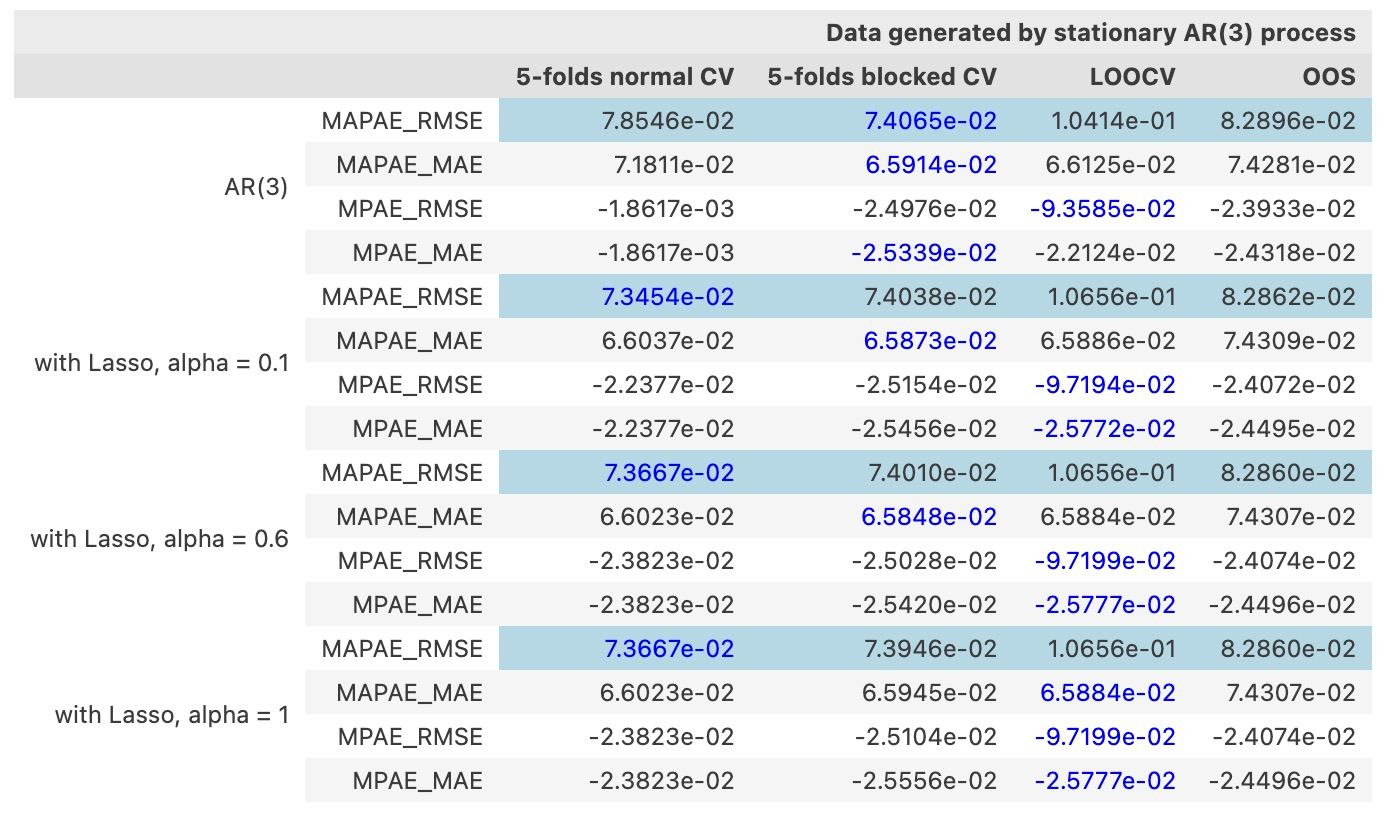
\includegraphics[scale=0.3]{Figures/ar3data_ar3.jpg}
    \label{ar3data_ar3}
\end{figure}
\FloatBarrier

\begin{figure}[hbt!]
    \caption{Experiment 2}
    \centering
    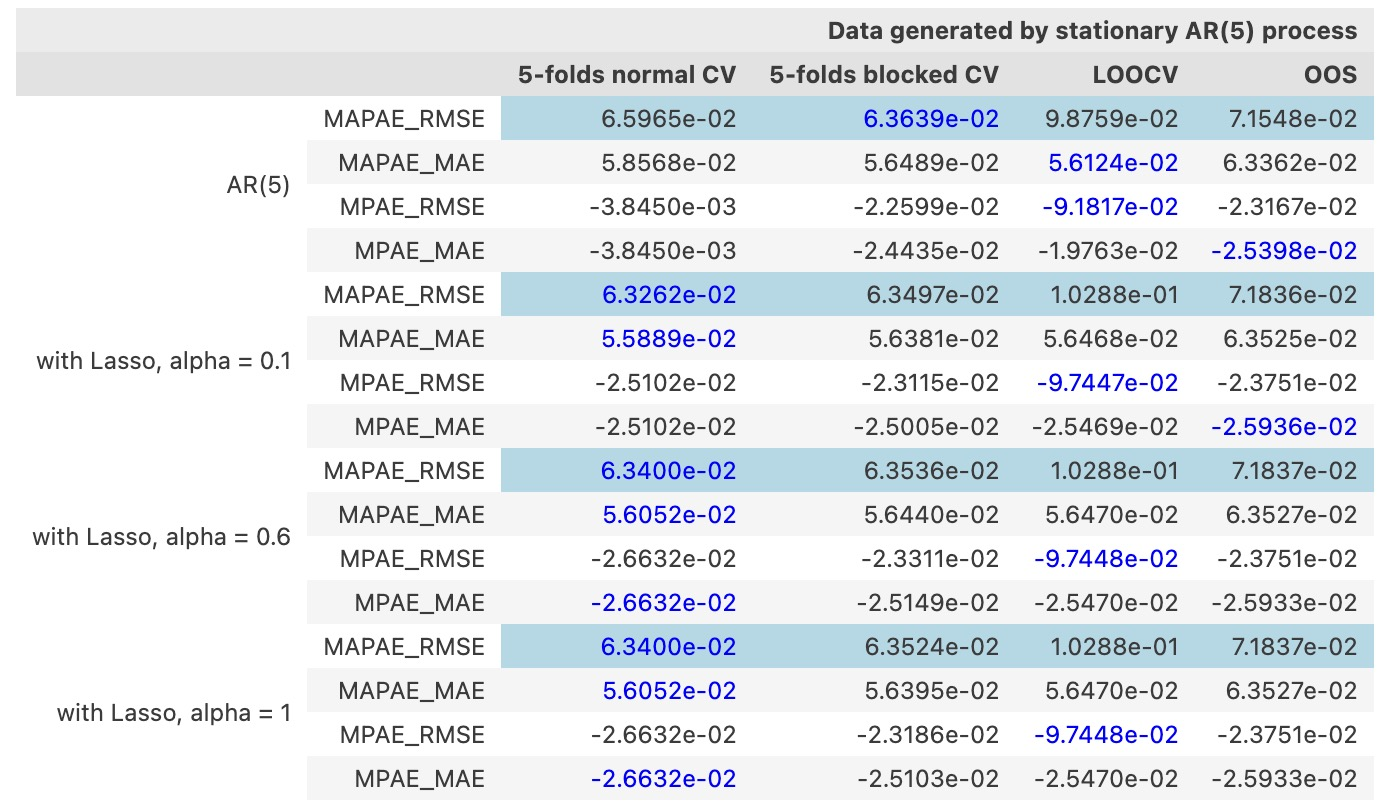
\includegraphics[scale=0.3]{Figures/ar5data_ar5.jpg}
    \label{ar5data_ar5}
\end{figure}
\FloatBarrier

\begin{figure}[hbt!]
    \caption{Experiment 3}
    \centering
    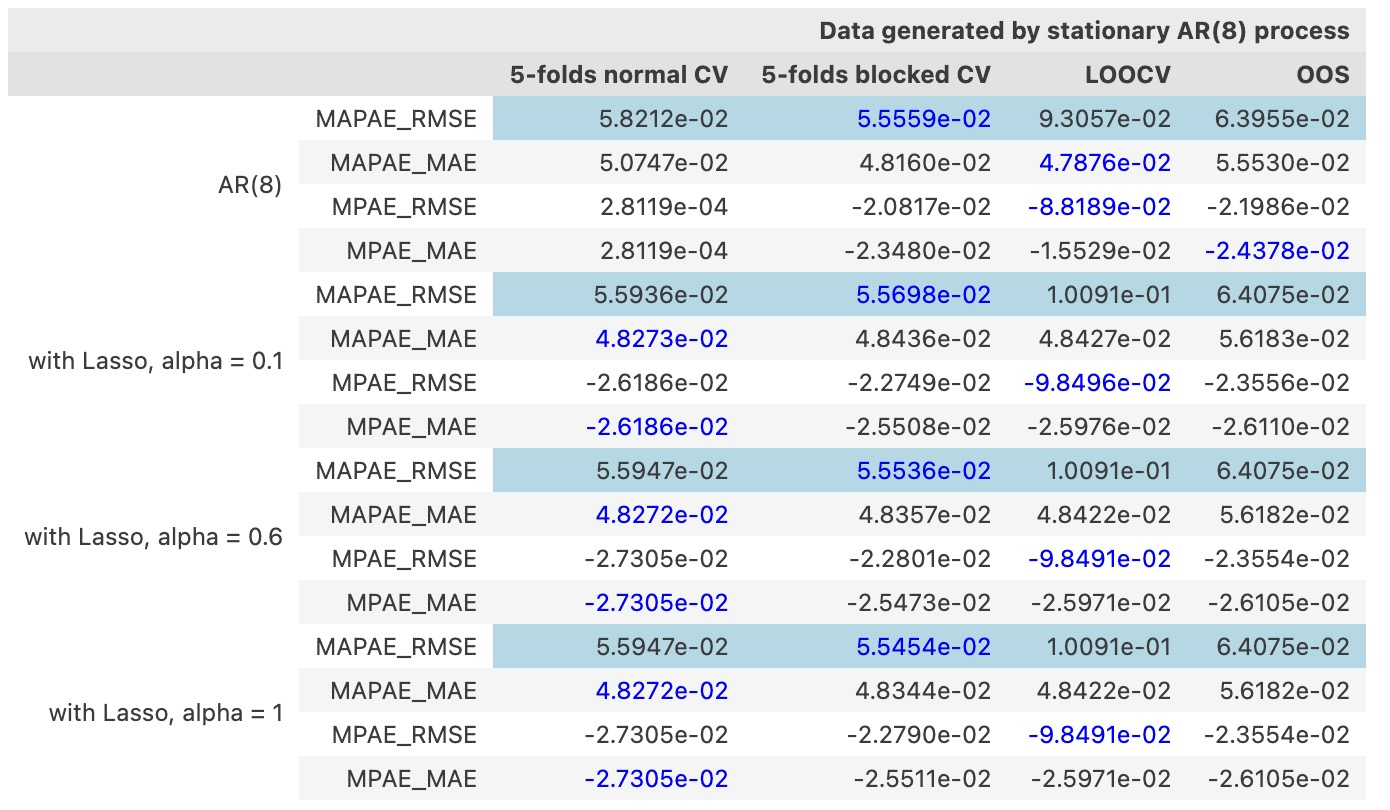
\includegraphics[scale=0.3]{Figures/ar8data_ar8.jpg}
    \label{ar8data_ar8}
\end{figure}
\FloatBarrier


\subsection{Future Improvements}
We can extend our study for future improvements in several different aspects and directions. In this section, we discuss four potential improvements to our current experimental design and methodology. These improvements aim to address limitations in model selection, regularization techniques, and cross-validation methods when applied to time series models, aiming for better generalization and more robust error estimation. 
\\
\\
\underline{Choice of Lasso Parameters}:
Besides testing with a limited and fixed set of $\alpha$ values as we did in our experiments, we can also use cross-validation within the in-set data to automatically select the optimal $\alpha$ value. And we can simulate the process for each Monte Carlo trial to see if a general range of $\alpha$ values out-performs for the chosen fitting model. 
\\
\\
\underline{Extension to Ridge Regression}: Ridge regression is another regularization technique like Lasso, but instead of penalizing the sum of the absolute values of the coefficients (Lasso), Ridge regression penalizes the sum of the squared values of the coefficients. The key difference is that Ridge regression introduces L2 regularization, which shrinks coefficients but does not necessarily set them to zero (as Lasso might do). We can use similar experiments set-up to compare with the results of Lasso regression.
\\
\\
\underline{Extension to Other Time Series Models}: We can extend our simulation to different time series models for data generation process and fitting procedure. However, when using complex models, we should always check if they meet the required assumptions. 
\\
\\
\underline{Other Error Metrics}:
We can explore using different error measures on in-set cross validation and out-set data. During the experiment, a vast range of values for \textbf{RMSE} and \textbf{MAE} was obtained when using different scaling factors in the time series data. Using other error measures like percentage errors in the experiments could provide a more standardized way of evaluating performance, as it normalizes the error relative to the data's value range. We can also explore additional error measures such as \textbf{BIC} or \textbf{AIC} to see how the complexity of the model affects the generalization error across different fitting methods. We can investigate on how much regularization or model selection improves the model’s ability to generalize.
\\
\\
\underline{Model Interpretability}:
As Lasso can drive some coefficients to zero, it would be interesting to track how many coefficients are reduced to zero across trials. This would provide some insights on how effective Lasso is and if there is any interpretability benefit such as identifying irrelevant lags. We can extend the experiments to models with higher lag values and on real-world data as well. 

\clearpage
\printbibliography
\end{document}

